\documentclass[11pt,english]{article}
\usepackage[T1]{fontenc}
\usepackage{babel}
\usepackage{graphicx}
\usepackage{hyperref}
\usepackage{rotating}
\usepackage{amsfonts}
\usepackage{amssymb}
\usepackage{listings}
\usepackage{color}
\usepackage{amsmath}
\usepackage{titlesec}
 
\setcounter{secnumdepth}{4}

\titleformat{\paragraph}
{\normalfont\normalsize\bfseries}{\theparagraph}{1em}{}
\titlespacing*{\paragraph}
{0pt}{3.25ex plus 1ex minus .2ex}{1.5ex plus .2ex}

 
\definecolor{codegreen}{rgb}{0,0.6,0}
\definecolor{codegray}{rgb}{0.5,0.5,0.5}
\definecolor{codepurple}{rgb}{0.58,0,0.82}
\definecolor{backcolour}{rgb}{0.95,0.95,0.92}
 
\lstdefinestyle{mystyle}{
    backgroundcolor=\color{backcolour},   
    commentstyle=\color{codegreen},
    keywordstyle=\color{magenta},
    numberstyle=\tiny\color{codegray},
    stringstyle=\color{codepurple},
    basicstyle=\footnotesize,
    breakatwhitespace=false,         
    breaklines=true,                 
    captionpos=b,                    
    keepspaces=true,                 
    numbers=left,                    
    numbersep=5pt,                  
    showspaces=false,                
    showstringspaces=false,
    showtabs=false,                  
    tabsize=2
}

\lstset{style=mystyle}

\begin{document}
\title{\textit{Deterministic DSA fault attack}}
\author{
  Fabio Gritti\\
  \texttt{fabio1.gritti@mail.polimi.it}
  \and
  Sebastiano Mariani\\
  \texttt{sebastiano.mariani@mail.polimi.it}
  \and \\
  \textbf{Professors}: Gerardo Pelosi , Alessandro Barenghi
}
\date{}
\maketitle

\pagestyle{plain}
\tableofcontents

\section{Introduction}
In this paper we want to introduce two active side channel attacks against the deterministic version of the Digital Signature Algorithm ( from now on DDSA ) as specified in the RFC 6979\cite{rfc}.\\
These attacks can lead directly to a leak of the private key and therefore breaking the authenticity of the signatures created using this algorithm. \\\\
We will proceed in this way: first we provide some useful background in order to understand better the paper, then we explain the attacks in details and finally we present the feasibility of the attack by showing the time needed to break the DSA with some of the keysize currently available.

\section{Background}

\subsection{The Digital Signature Algorithm}

\subsubsection{General overview}
The DSA is one of three digital signature schemes specified in FIPS 186\cite{fips}. A digital signature scheme is an authentication mechanism that enables the creator of a message to attach a code that acts as a signature providing authenticity and non-repudation. \\It usually consists of three algorithms:

\begin{itemize}
\item a \textit{key generation algorithm} that outputs the private key and the corresponding public key.
\item a \textit{signing algorithm} that given a message and a private key produce the signature. 
\item a \textit{signature verifying algorithm} that given a signature and a public key either accepts or rejects the message's claim to authenticity.
\end{itemize}

In order to be a sound digital signature schemes the following properties must hold:

\begin{itemize} 
\item the authenticity of a signature generated from a fixed message and fixed private key can be verified by using the corresponding public key.
\item it should be computationally infeasible to generate a valid signature for a party without knowing that party's private key. 
\item The private key MUST remain private, otherwise the authenticity of the signature created with that key is broken.
\item The public key owner MUST be verifiable, otherwise we can't assure that we had receive a message from a particoular source.
\end{itemize}

\subsubsection{DSA mathematical structure}

The reference group category is $(\mathbb{Z}^{*}_{p},\cdot )$ , \textit{p} prime s.t. \textit{q} | ( \textit{p-1} )} with \textit{q} also prime. The employed algebraic structure is then the multiplicative cyclic subgroup \textit{G} = <\textit{g}> with publicly known generator \textit{g} and order \textit{q}.

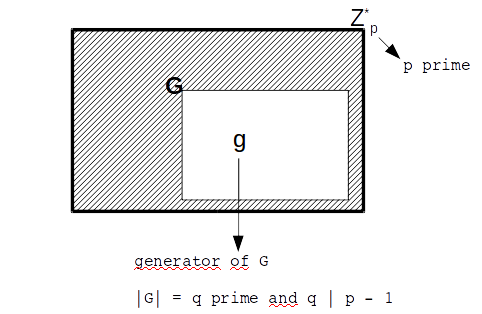
\includegraphics[width=0.8\textwidth]{img/img_1.png} \\ 

FIPS 186-3 specifies the (L = $log_{2}(p)$ N = $log_{2}(q)$ ) length pairs of (1024,160),(2048,224),(2048,256) and (3072,256).

\subsubsection{Cryptoscheme}

Public  Key: $k_{pub} = (p,q,g,g^s)$ \\
Private Key: $k_{priv} = s \in \mathbb{Z}^{*}_{q}$
\\\\\\\\\\\\
Signature Transformation:\\
\framebox[9cm]{
\begin{minipage}{8cm}
$H(m)\in \{2,...,q-1\}$\\
$k \overset{random}{\leftarrow}\mathbb{Z}^{*}_{q}$\\
r \leftarrow ((g^l) $mod p$)$mod q$\\
if  $r = 0 repeat with another random l$ \\
s \leftarrow $k^{-1} \cdot (H(m) - s*r)$ $mod q $\\
if $s = 0$ , repeat with another random $k$\\\\
$Signature = < s,r >$\\
$Send(m,Signature)$\\
\end{minipage}
}
\\\\\\\\
Validation Check:\\
\framebox[9cm]{
\begin{minipage}{8cm}
\\Receive <m,Signature>\\
if r,s $\notin \{1,....,q-1\}$  reject the signature
Compute H(m)\\
\\
Accept signature if:\\
u_{1} \leftarrow H(m)\cdot s^{-1} $mod q$ \\
u_{2} \leftarrow r \cdot s^{-1} $mod q$ \\
(g^{u_{1}}((g^{s})^{u_{2}}) $mod p mod q$ == r ?\\
\end{minipage}
}




\subsection{The Deterministic Digital Signature Algorithm}

\subsubsection{General overview}
The step in the signing algorithm that require to generate a random parameter needs a great randomness in order to be secure; but digging with embedded system not always we have on board a sound RNG! \\This is the crucial point for which many manufacturers decide to employ RSA cryptosystem rather than DSA/ECDSA to sign objects.\\
\\The Deterministic DSA proposed in the RFC 6979 try to make that step deterministic ( and impossible to deduct without the private key ) in order to increase the attractiveness of such system in the embedded world ( smart card, credit card , console, ... ).\\\\
Remember that we ,in any way, need a good RNG in order to generate a strong private key. 
This proposal make deterministic the signing, NOT the generation of keys that MUST be non deterministic and made a priopri.


\subsubsection{K deterministic generation}

The generation of the deterministic \textit{k} depends only from the message to sign and the private key.\\
According to the RFC ,  given the input message m, the following process is applied for the generation:

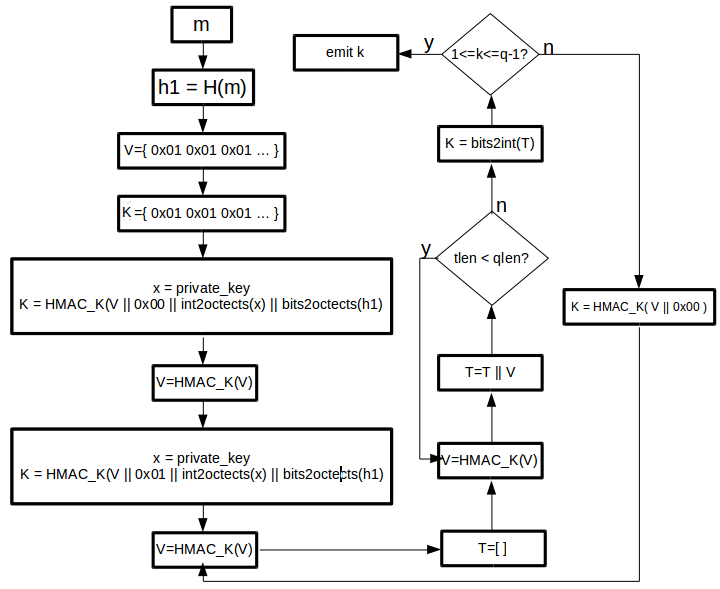
\includegraphics[width=1.0\textwidth]{img/img_2.png} \\

\begin{itemize}
\item qlen = binary length of the prime number \textit{q}
\item tlen = binary length of the array T 
\item The internal HMAC use the same hash function used in the h1=H(m)
\end{itemize}

\subsection{Other digital signature algorithm}

Chosing a different group and a different set of operations it is possible to build some variant of the DSA algorithm.The two principal cìvariants are:
\begin{itemize}
	\item \textbf{dECDSA:}
	Is a variant of DSA which uses elliptic curve cryptography. With this type of cryptography is possible to achive the same security level, compared to the normal DSA algorithm, with a smaller key length.
	\item \textbf{EdDSA Bernstein:}
The Edwards-curve digital sign algorithm is a digital signature scheme using a variant of Schnorr signature based on Twisted Edwards curves. It is designed for high performance while avoiding security problems that have surfaced in other digital signature schemes such as some side channel attack.
\end{itemize}

\section{Cracking the Deterministic DSA}

\subsection{Differential fault analysis}

The differential fault analysis is an active side channel attack that is performed in three steps:
\begin{itemize}
\item Obtain the correct signature of a message.
\item Inject a fault during a second signing of the message and obtain the \textit{faulty signature}.
\item Correlate the correct signature with the faulty one and extract the private key.
\end{itemize}

In order to inject a fault we can use different techniques that range from using laser beam during the signing process, to voltage spike, insane overclocking etc..
\\Usually critical embedded systems like credit card implements different defenses against this fault injection techniques; this raise a lot the cost of an attack performed by an attacker. \\Bypass this kind of defense is out of scope of this paper.

\subsection{The attack in practice}

We test our attack against the implementation of the DSA RFC 6979 in the GNU/libgcrypt\cite{lib} library. 
In order to inject the attack using the library we added a flag during the building of the s-expression relative to the plaintext e.g.:

\begin{lstlisting}
err = gcry_sexp_build(&ptx2, NULL, "(data (flags rfc6979) (hash %s %b) (attack2))" , "sha1", hash_len , digest);
\end{lstlisting}

When the function dsa-sign find that flag it redirects the flow to our faulty function that injects the desidered fault based on the type of the attack we want to perform.

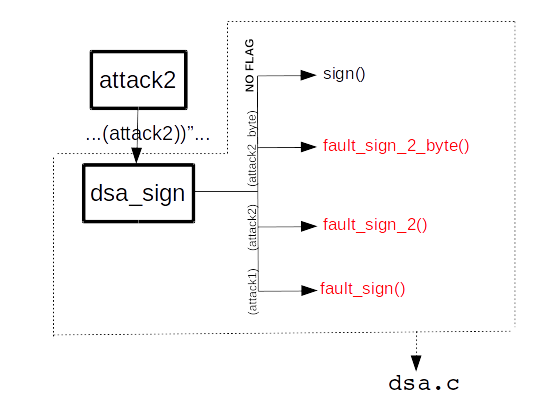
\includegraphics[width=1.0\textwidth]{img/img_3.png} \\

The next two paragraphs describe the two attacks type and then we present the result obtained.

\subsubsection{Damage the exponentation}

Remembering from the DDSA scheme that we have to exponentiate the generator \textit{g} at the power of \textit{k}, we inject a bit fault into k during the exponentiation, obtaining g^{\tilde{k}} = \tilde{r} = r \cdot g^{\pm 2^{i}}.

\begin{lstlisting}

  [ FROM /libgcrypt/cipher/dsa.c fault_sign function ]

  [...]
  
  gcry_mpi_t one = mpi_set_ui(NULL, 1);  

  gcry_mpi_t e = mpi_new(qbits);
  
  //calculate 2^bit_fault
  mpi_mul_2exp(e, one, (unsigned long)bit_fault); 

  gcry_mpi_t k_tilde = mpi_new(qbits);

  //damage the k 
  if( sign == 0 ) 
     mpi_subm(k_tilde,k,e,skey->q); 
  else 
     mpi_addm(k_tilde,k,e,skey->q);

  mpi_mul(sig_k, k_tilde, one);
  
  //****************** FAULT *********************//
  mpi_powm( r, skey->g, k_tilde, skey->p );  
  mpi_fdiv_r( r, r, skey->q );    
  //****************** FAULT *********************//
  
  
  [ ... ] 
\end{lstlisting}

The attacks proceeds as follows:
\begin{itemize}
\item Obtain the correct signature $s = k^{-1}(m + xr) $
\item Obtain the faulty signature $\tilde{s} = k^{-1}(m + x\tilda{r})$
\item Write the system:\\ \\\begin{cases} s = k^{-1}(m + xr) \\ \tilde{s} = k^{-1}(m + x\tilde{r}) \end{cases}\\
\\with \textit{k} and \textit{x} are unknown.


\item Solving,we  obtain:\\\\
\begin{cases}
x \equiv_{q} \frac{(s-\tilde{s})m}{(r\tilde{s} - \tilde{r}s)} \\
k \equiv_{q} s^{-1}(mx+r)
\end{cases}

\end{itemize}


This attack is very interesting because it doesn't need any bruteforce in order to discover the key: all the parameters that we need in the previous formula are available from the output of the correct and faulty algorithm.

The correctness of the attack is checked by creating a new dsa-key-pair based on the private key calculated and by signing a new plaintext with that key and then try to verify the signature with the original public key.


\subsubsection{Damage the signature composition}

For this attack we consider two level: a bit level and a byte level.\\\\ The bit level assume that with an active side channel attack we can surgically flip a single bit of k during the signature composition; this assumption is really optimistic and this precision can lead to a very fast cracking during the bruteforcing part of the algorithm.\\\\ The byte level is a more realistic assumption that we inject a fault of a byte inside the k; in this case the bruteforcing part of the attack will be slower , but the cost in order to inject the fault pratically is reduced.

\paragraph{Bit level fault}

\begin{lstlisting}
 
  [ FROM /libgcrypt/cipher/dsa.c fault_sign_2 function ]

  [...]
  
  mpi_powm( r, skey->g, k, skey->p );
  mpi_fdiv_r( r, r, skey->q );

  gcry_mpi_t one = mpi_set_ui(NULL, 1); 

  //calculat 2^i ()
  gcry_mpi_t e = mpi_new(qbits);
  mpi_mul_2exp(e, one, (unsigned long) bit_fault);  

  gcry_mpi_t k_tilde = mpi_new(mpi_get_nlimbs(k));
  

  //damage the k
  if(sign==0)
     mpi_subm(k_tilde,k,e,skey->q);  
  else
     mpi_addm(k_tilde,k,e,skey->q);

  //****************** FAULT *********************//
  
  mpi_mul(sig_k, k_tilde, one);
  
  kinv = mpi_alloc( mpi_get_nlimbs(k) );
  mpi_invm(kinv, k_tilde, skey->q );
  
  //****************** FAULT *********************//
  
 [...]

\end{lstlisting}

The attacks with a bit fault proceeds as follows: 
\begin{itemize}
\item Obtain the correct signature $s = k^{-1}(m + xr) $
\item Obtain the faulty signature $\tilde{s} = \tilde{k}^{-1}(m + xr)$
\item Notice that \\$\frac{s}{\tilde{s}}  = \frac{k^{-1}(m+xr)}{\tilde{k}^{-1}(m+xr)}$

\item In case of a negative fault $k-2^{i} $ we have\\ $\frac{s}{\tilde{s}} = \frac{k^{-1}(m+xr)}{(k-2^{i})^{-1}(m+xr)}$

\item In case of a positive fault $k+2^{i} $ we have \\$\frac{s}{\tilde{s}} = \frac{k^{-1}(m+xr)}{(k+2^{i})^{-1}(m+xr)}$


\item calulating k for both the case we have: \\$k_{faultpos} = \frac{\tilde{s}2^{i}}{s-\tilde{s}}$ \\
$k_{faultneg} = \frac{\tilde{s}2^{i}}{\tilde{s}-s}$ \\

\item Notice that in this case we need a bruteforce in order to discover the right \textit{i} ( which bit has been flipped, 0<=i<=qbits ) and so to finally calculate k

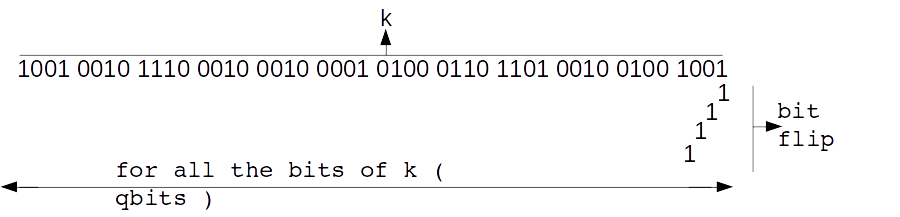
\includegraphics[width=1.0\textwidth]{img/img_5.png} \\

\item After discovered the k, we can calculate the private key x as:\\ $x = \frac{sk - m}{r}$

\end{itemize}

\paragraph{Byte level fault}

\begin {lstlisting}

  [ FROM /libgcrypt/cipher/dsa.c   fault_sign_2_byte function ]
  
  [ ... ]
  
  mpi_powm( r, skey->g, k, skey->p );
  mpi_fdiv_r( r, r, skey->q );

  gcry_mpi_t one = mpi_set_ui(NULL, value_fault);   


  gcry_mpi_t e = mpi_new(qbits);
  mpi_mul_2exp(e, one, byte_fault);   

  gcry_mpi_t k_tilde = mpi_new(mpi_get_nlimbs(k));

  if(sign==0)
     mpi_subm(k_tilde,k,e,skey->q);  
  else
     mpi_addm(k_tilde,k,e,skey->q);

  //****************** FAULT *********************//
  
  mpi_mul(sig_k, k_tilde, one);
  
  kinv = mpi_alloc( mpi_get_nlimbs(k) );
  mpi_invm(kinv, k_tilde, skey->q );

  //****************** FAULT *********************//
  
  [ ... ]

\end{lstlisting}

The attacks with a byte fault proceeds as follows: 
\begin{itemize}
\item Obtain the correct signature $s = k^{-1}(m + xr) $
\item Obtain the faulty signature $\tilde{s} = \tilde{k}^{-1}(m + xr)$
\item Notice that \\$\frac{s}{\tilde{s}}  = \frac{k^{-1}(m+xr)}{\tilde{k}^{-1}(m+xr)}$

\item In case of a negative fault $k-b2^{i} $ we have\\ $\frac{s}{\tilde{s}} = \frac{k^{-1}(m+xr)}{(k-b2^{i})^{-1}(m+xr)}$

\item In case of a positive fault $k+b2^{i} $ we have \\$\frac{s}{\tilde{s}} = \frac{k^{-1}(m+xr)}{(k+b2^{i})^{-1}(m+xr)}$


\item calulating k for both the case we have: \\$k_{faultpos} = \frac{\tilde{s}b2^{i}}{s-\tilde{s}}$ \\
$k_{faultneg} = \frac{\tilde{s}b2^{i}}{\tilde{s}-s}$ \\

\item Notice that in this case we need a bruteforce in order to discover the right \textit{b} and \textit{i} ( which byte has been flipped, 0<=i<=qbits and the value of the fault b, 0<=b<=255) and so to finally calculate k. The index \textit{i} is the value of the shift of the fault value b (we are trying all the possible value, for all the possible shift).

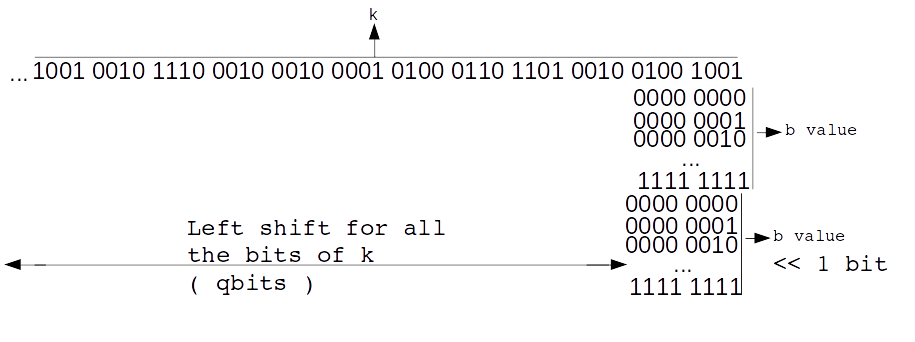
\includegraphics[width=1.0\textwidth]{img/img_4.png} \\

\item After discovered the k, we can calculate the private key x as:\\ $x = \frac{sk - m}{r}$


\end{itemize}
\section{Results}
We have tested these attack on 4 key length:
\begin{itemize}
\item p = 1024 bit		q = 160 bit
\item p = 2048 bit		q = 224 bit
\item p = 2048 bit		q = 256 bit
\item p = 3072 bit 		q = 256 bit
\end{itemize}
And with two scenarios for each length:
\begin{itemize}
\item optimal case: the fault happens on the first bit/byte of k 
\item worst case: the fault happens on the last bit/byte of k
\end{itemize}

\subsection{Damage the exponentation}
\begin{itemize}
\item Bit level \ Byte level:

In this attack the distincton between bit level and byte level has no meaning because the time complexity is alway O(c) regardless the type of the fault injected. The private key is cracked in less than one second even if the fault is injected at the word level.

\end{itemize}


\subsection{Damage the signature composition}
\begin{itemize}
\item Bit level:

\begin{table}[!htbp]
\centering
\label{my-label}
\begin{tabular}{|c|c|c|}
\hline
         & Optimal case & Worst case     \\ \hline
Length 1 & 4.953000 ms  & 295.578003 ms  \\ \hline
Length 2 & 14.788000 ms & 1547.551025 ms \\ \hline
Length 3 & 15.799001 ms & 2021.688965 ms \\ \hline
Length 4 & 28.413000 ms & 3562.698975 ms \\ \hline
\end{tabular}
\end{table}


\item Byte level:
\begin{table}[!htbp]
\centering
\label{my-label}
\begin{tabular}{|c|c|c|}
\hline
         & Optimal case & Worst case     \\ \hline
Length 1 & 132.716995 ms  & 75677.210938 ms  \\ \hline
Length 2 & 479.232025 ms & 290135.656250 ms \\ \hline
Length 3 & 555.675049 ms & 447803.687500 ms \\ \hline
Length 4 & 972.052002 ms & 841949.000000 ms \\ \hline
\end{tabular}
\end{table}


\end{itemize}


\section{Conclusion}

\addcontentsline{toc}{section}{\refname}
\begin{thebibliography}{10}
\bibitem{rfc} https://tools.ietf.org/html/rfc6979
\bibitem{fips} http://nvlpubs.nist.gov/nistpubs/FIPS/NIST.FIPS.186-4.pdf
\bibitem{lib}https://www.gnu.org/software/libgcrypt/
\end{thebibliography}

\end{document}
